\chapter{Introduction}

% 1) paralalicia vseobecne
These days, we are increasingly encountering parallel programs.
A dozen programs that have been written in a typical way for single-core systems cannot take advantage of the presence of computers with multiple cores.
When we wanted to speed up problem-solving, we wanted to create something that would eliminate our time on calculations.
Thus, we invented the computer, which knew relatively nothing to do at the beginning.
However, after a few years, all this changed, and the computer solved problems that took a person many days.
Nowadays, we live in a time when computers have significantly improved execution time by solving different problems using parallelism.

% 2) úvod do problematiky
Several years ago, \emph{Google} released a technology that defined and changed our application deployment and management perspective.
An iterative sequence of small steps caused this revolution (i.e., physical, virtual and container era).
\emph{Kubernetes}~\cite{history, kubernetes, kubernetesBook} is a container management system, and in another mini-iteration, brought a new concept of how to organise containers more efficiently \---\ the \emph{Operator pattern}.
\emph{Operator pattern} aims to capture how to extend and implement automation tasks beyond \emph{Kubernetes}.
One such Operator is developed and maintained as part of an open-source project called Strimzi~\cite{strimziDoc, strimziBlogPosts}.
The \emph{Strimzi} project brings together several tools that take care of   Apache Kafka~\cite{apacheKafkaDefinitiveGuide, apacheKafkaDesignDistributedSystems, kafkaStreamsBook, kafkaDocumentation} deployment on Kubernetes.
Complexity, horizontal scalability and distribution system;
are all attributes of \emph{Apache Kafka}.
Unfortunately, these attributes make the system an exceedingly complex entity to verify.
Therefore, one of the biggest challenges of using \emph{Kubernetes} is effectively and quickly testing projects like \emph{Kafka} and \emph{Strimzi} while verifying integration with similar products (i.e.,
\emph{Prometheus}\footnote{Prometheus \---\ open-source metrics-based project. Moreover, it provides an alerting system with incredible features, in case of interest \url{https://prometheus.io/}},
Grafana\footnote{Grafana \---\ open-source project, which primary responsibility is to show user interactive visualisation to track crucial parts of the system via the great user interface. (\url{https://grafana.com/})},
Jaeger\footnote{Jaeger (Jaeger Tracing) \---\ is a product which finds and helps troubleshoot problems in distributive systems. (\url{https://www.jaegertracing.io/})},
Keycloak\footnote{Keycloak \---\ open-source project for securing applications (authentication and authorization). (\url{https://www.keycloak.org/})}).
Regarding the resources required to deploy \emph{Kafka} on virtual machines or containers, it is relatively simple to compare Kafka's Deployment on \emph{Kubernetes}.
Nevertheless, this causes time problems for our \emph{Strimzi} project testing.
To solve this problem, we have adopted the principles of parallel execution and created a mechanism within the \emph{Strimzi system tests}, which runs tests in parallel against only one cluster of \emph{Kubernetes}.

\bigskip
% 4) prínosy tejto práce

\textbf{Key Contributions} \quad Related work focuses on improving the overall verification time of a Strimzi product.
Several releases of Strimzi give us empirical insights that testing using a sequential computational model has been extremely slow.
Furthermore, the product contains about fifteen of the most critical possible combinations of product deployment, each of which lasts over sixty hours.
This sequential computational model is not a recommended candidate for verifying such numerous deployments.
An attentive reader could see the entire test time approaching one thousand hours, which is approximately one and a half month.
\begin{figure}[!ht]
    \centering
    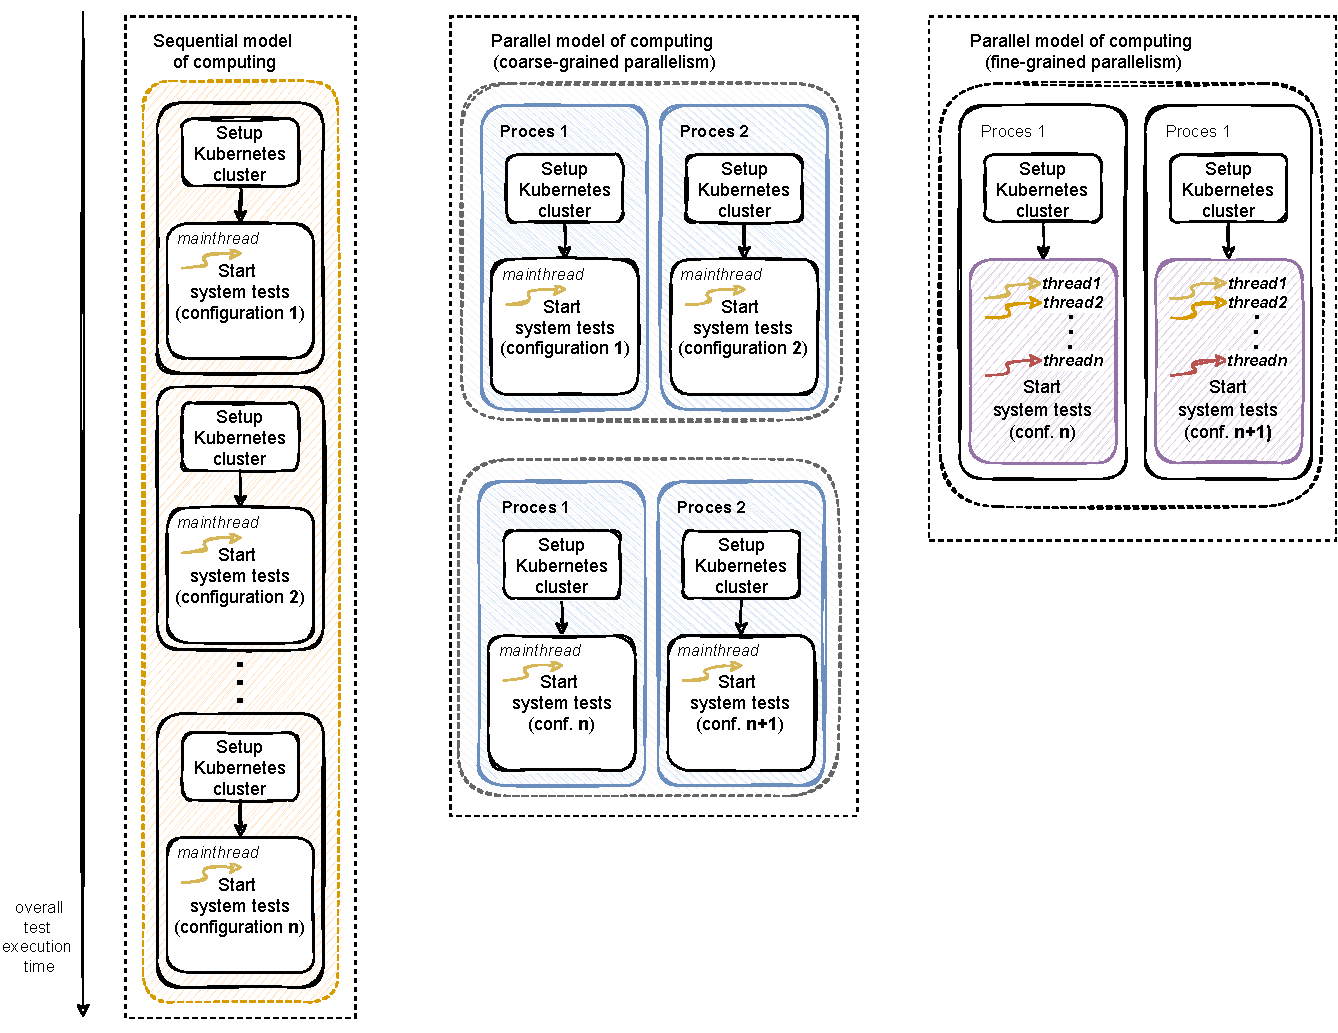
\includegraphics[scale=0.65]{obrazky-figures/01-intro/00-intro-better-one}
    \label{00:fig:evolution}
    \caption{Evolution of our test framework execution}
\end{figure}
Nevertheless, as part of this effort for coarse-grained parallelism in performing multiple product deployments, it partially accelerated the overall computation.
However, this approach is not horizontally scalable due to our cloud services that provide resources (i.e., bare metals, virtual machines, containers).
Therefore, we got to the last opportunity to improve the computation using the vertical scalability of the resources (i.e., memory, central processing units) that the cloud services offer us.
This information motivated us to design and implement a mechanism of fine-grained parallelism in our test framework.
Figure~\ref{00:fig:evolution} shows the overall evolution of our test framework and summarises the previously mentioned sentences.
The experiments on the implementation show that the given parallelization can significantly improve the execution time.
% tak celkovú verifikáciu zlepšiť z 1000h na viac ako polovicu (i.e., ~350h).
The author contributed the given code to the open-sourced project Strimzi, available on Github\footnote{Strimzi Github repository \---\ \url{https://github.com/strimzi/strimzi-kafka-operator}}, which also makes it possible to inspire other \emph{kube-native}\footnote{Kube-native \---\ it is a product that has been moved from the standalone world to the Kubernetes world. Moreover, it provides a communication interface (i.e., Kubernetes REST API) with which it manages individual components (i.e., Apache Kafka is a standalone application, and Strimzi is a \emph{kube-native} product because it encapsulates Apache Kafka and provides a communication interface for the user.} products to implement such solutions.
The comprehensive benefit of this work is the acceleration of the verification process.

\bigskip
% 5) štruktúra práce

\textbf{The structure of the diploma thesis} \quad The author decomposed the whole work into seven chapters together with an introduction.
In Chapter~\ref{02:chapter:title}, the reader learns about the theoretical background to understand the overall thesis (i.e., Kubernetes, Apache Kafka, Strimzi).
Subsequently, we explain the fundamental concepts of parallelism (i.e., Amdahl's law (\ref{04:amdalhlaw}), Shared memory (\ref{04:sharedmemory}), Process and Thread (\ref{04:processesandthreads}), Synchronisation (\ref{04:synchronization}) in Chapter~\ref{03:chapter:title}.
Chapter~\ref{04:chapter:title} presents bottlenecks in the current approach to testing the Strimzi product and proposes a brand-new computational architecture that solves many issues.
Moreover, in Chapter~\ref{05:chapter:title}, we describe the implementation of the proposed architecture.
In the penultimate part of this thesis (Chapter~\ref{06:chapter:title}), we summarise the results from many experiments with a deep analysis of the thesis implementation.
Finally, we conclude the entire diploma thesis with the knowledge that has been acquired in Chapter~\ref{08:chapter:title}.